% This file was created with matplot2tikz v0.5.3.
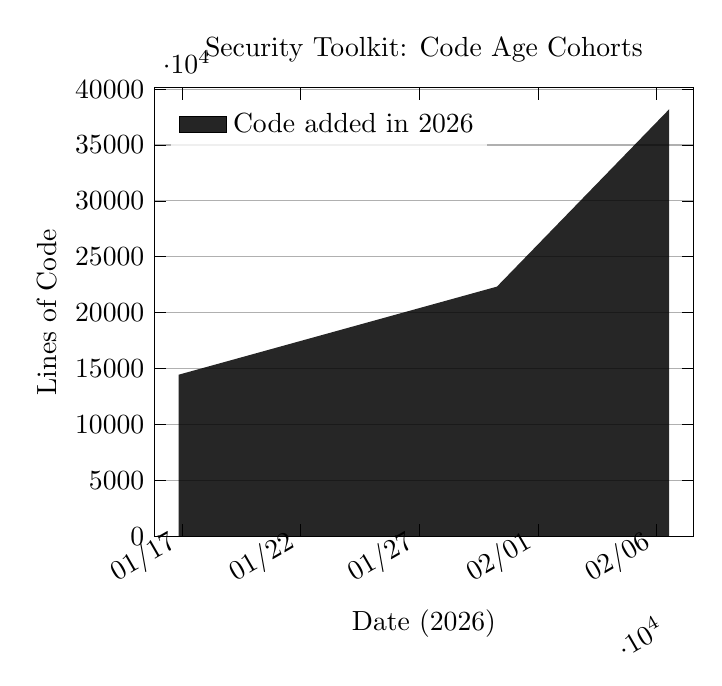
\begin{tikzpicture}

\definecolor{darkgray176}{RGB}{176,176,176}

\begin{axis}[
legend cell align={left},
legend style={
  fill opacity=0.8,
  draw opacity=1,
  text opacity=1,
  at={(0.03,0.97)},
  anchor=north west,
  draw=none
},
tick pos=both,
title={Security Toolkit: Code Age Cohorts},
x grid style={darkgray176},
xlabel={Date (2026)},
xmin=20468.8295462963, xmax=20491.5690416667,
xtick style={color=black},
xtick={20465,20470,20475,20480,20485,20490,20495},
xticklabel style={rotate=30.0,anchor=east},
xticklabels={01/12,01/17,01/22,01/27,02/01,02/06,02/11},
y grid style={darkgray176},
ylabel={Lines of Code},
ymajorgrids,
ymin=0, ymax=40112.1,
ytick style={color=black},
ytick={0,5000,10000,15000,20000,25000,30000,35000,40000,45000},
yticklabels={
  \(\displaystyle {0}\),
  \(\displaystyle {5000}\),
  \(\displaystyle {10000}\),
  \(\displaystyle {15000}\),
  \(\displaystyle {20000}\),
  \(\displaystyle {25000}\),
  \(\displaystyle {30000}\),
  \(\displaystyle {35000}\),
  \(\displaystyle {40000}\),
  \(\displaystyle {45000}\)
}
]
\path [fill=black, fill opacity=0.85]
(axis cs:20469.8631597222,14447)
--(axis cs:20469.8631597222,0)
--(axis cs:20483.27875,0)
--(axis cs:20490.5354282407,0)
--(axis cs:20490.5354282407,38202)
--(axis cs:20490.5354282407,38202)
--(axis cs:20483.27875,22331)
--(axis cs:20469.8631597222,14447)
--cycle;
\addlegendimage{area legend, fill=black, fill opacity=0.85}
\addlegendentry{Code added in 2026}

\end{axis}

\end{tikzpicture}
